% Created by tikzDevice version 0.12.3.2 on 2022-07-13 10:39:42
% !TEX encoding = UTF-8 Unicode
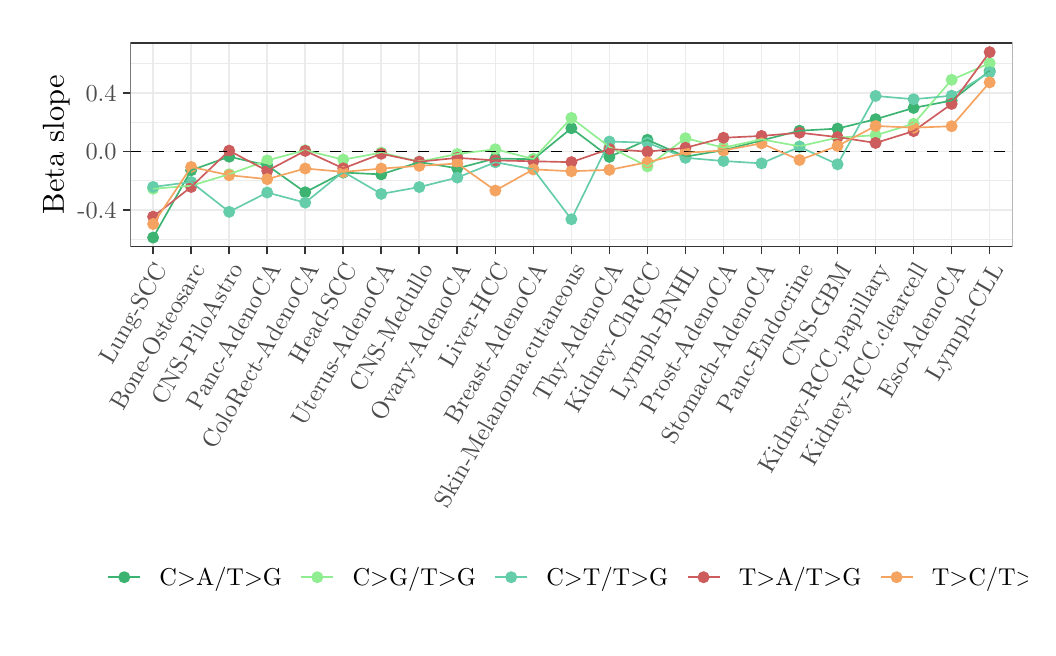
\begin{tikzpicture}[x=1pt,y=1pt]
\definecolor{fillColor}{RGB}{255,255,255}
\path[use as bounding box,fill=fillColor,fill opacity=0.00] (0,0) rectangle (361.35,216.81);
\begin{scope}
\path[clip] (  0.00,  0.00) rectangle (361.35,216.81);
\definecolor{drawColor}{RGB}{255,255,255}
\definecolor{fillColor}{RGB}{255,255,255}

\path[draw=drawColor,line width= 0.6pt,line join=round,line cap=round,fill=fillColor] (  0.00,  0.00) rectangle (361.35,216.81);
\end{scope}
\begin{scope}
\path[clip] ( 37.09,137.61) rectangle (355.85,211.31);
\definecolor{fillColor}{RGB}{255,255,255}

\path[fill=fillColor] ( 37.09,137.61) rectangle (355.85,211.31);
\definecolor{drawColor}{gray}{0.92}

\path[draw=drawColor,line width= 0.3pt,line join=round] ( 37.09,140.26) --
	(355.85,140.26);

\path[draw=drawColor,line width= 0.3pt,line join=round] ( 37.09,161.47) --
	(355.85,161.47);

\path[draw=drawColor,line width= 0.3pt,line join=round] ( 37.09,182.67) --
	(355.85,182.67);

\path[draw=drawColor,line width= 0.3pt,line join=round] ( 37.09,203.87) --
	(355.85,203.87);

\path[draw=drawColor,line width= 0.6pt,line join=round] ( 37.09,150.86) --
	(355.85,150.86);

\path[draw=drawColor,line width= 0.6pt,line join=round] ( 37.09,172.07) --
	(355.85,172.07);

\path[draw=drawColor,line width= 0.6pt,line join=round] ( 37.09,193.27) --
	(355.85,193.27);

\path[draw=drawColor,line width= 0.6pt,line join=round] ( 45.33,137.61) --
	( 45.33,211.31);

\path[draw=drawColor,line width= 0.6pt,line join=round] ( 59.07,137.61) --
	( 59.07,211.31);

\path[draw=drawColor,line width= 0.6pt,line join=round] ( 72.81,137.61) --
	( 72.81,211.31);

\path[draw=drawColor,line width= 0.6pt,line join=round] ( 86.55,137.61) --
	( 86.55,211.31);

\path[draw=drawColor,line width= 0.6pt,line join=round] (100.29,137.61) --
	(100.29,211.31);

\path[draw=drawColor,line width= 0.6pt,line join=round] (114.03,137.61) --
	(114.03,211.31);

\path[draw=drawColor,line width= 0.6pt,line join=round] (127.77,137.61) --
	(127.77,211.31);

\path[draw=drawColor,line width= 0.6pt,line join=round] (141.51,137.61) --
	(141.51,211.31);

\path[draw=drawColor,line width= 0.6pt,line join=round] (155.25,137.61) --
	(155.25,211.31);

\path[draw=drawColor,line width= 0.6pt,line join=round] (168.99,137.61) --
	(168.99,211.31);

\path[draw=drawColor,line width= 0.6pt,line join=round] (182.73,137.61) --
	(182.73,211.31);

\path[draw=drawColor,line width= 0.6pt,line join=round] (196.47,137.61) --
	(196.47,211.31);

\path[draw=drawColor,line width= 0.6pt,line join=round] (210.21,137.61) --
	(210.21,211.31);

\path[draw=drawColor,line width= 0.6pt,line join=round] (223.95,137.61) --
	(223.95,211.31);

\path[draw=drawColor,line width= 0.6pt,line join=round] (237.69,137.61) --
	(237.69,211.31);

\path[draw=drawColor,line width= 0.6pt,line join=round] (251.43,137.61) --
	(251.43,211.31);

\path[draw=drawColor,line width= 0.6pt,line join=round] (265.17,137.61) --
	(265.17,211.31);

\path[draw=drawColor,line width= 0.6pt,line join=round] (278.91,137.61) --
	(278.91,211.31);

\path[draw=drawColor,line width= 0.6pt,line join=round] (292.65,137.61) --
	(292.65,211.31);

\path[draw=drawColor,line width= 0.6pt,line join=round] (306.39,137.61) --
	(306.39,211.31);

\path[draw=drawColor,line width= 0.6pt,line join=round] (320.13,137.61) --
	(320.13,211.31);

\path[draw=drawColor,line width= 0.6pt,line join=round] (333.87,137.61) --
	(333.87,211.31);

\path[draw=drawColor,line width= 0.6pt,line join=round] (347.61,137.61) --
	(347.61,211.31);
\definecolor{drawColor}{RGB}{60,179,113}
\definecolor{fillColor}{RGB}{60,179,113}

\path[draw=drawColor,line width= 0.4pt,line join=round,line cap=round,fill=fillColor] ( 59.07,165.28) circle (  1.96);
\definecolor{drawColor}{RGB}{144,238,144}
\definecolor{fillColor}{RGB}{144,238,144}

\path[draw=drawColor,line width= 0.4pt,line join=round,line cap=round,fill=fillColor] ( 59.07,159.68) circle (  1.96);
\definecolor{drawColor}{RGB}{102,205,170}
\definecolor{fillColor}{RGB}{102,205,170}

\path[draw=drawColor,line width= 0.4pt,line join=round,line cap=round,fill=fillColor] ( 59.07,161.04) circle (  1.96);
\definecolor{drawColor}{RGB}{205,92,92}
\definecolor{fillColor}{RGB}{205,92,92}

\path[draw=drawColor,line width= 0.4pt,line join=round,line cap=round,fill=fillColor] ( 59.07,159.25) circle (  1.96);
\definecolor{drawColor}{RGB}{244,164,96}
\definecolor{fillColor}{RGB}{244,164,96}

\path[draw=drawColor,line width= 0.4pt,line join=round,line cap=round,fill=fillColor] ( 59.07,166.48) circle (  1.96);
\definecolor{drawColor}{RGB}{60,179,113}
\definecolor{fillColor}{RGB}{60,179,113}

\path[draw=drawColor,line width= 0.4pt,line join=round,line cap=round,fill=fillColor] (182.73,169.27) circle (  1.96);
\definecolor{drawColor}{RGB}{144,238,144}
\definecolor{fillColor}{RGB}{144,238,144}

\path[draw=drawColor,line width= 0.4pt,line join=round,line cap=round,fill=fillColor] (182.73,169.38) circle (  1.96);
\definecolor{drawColor}{RGB}{102,205,170}
\definecolor{fillColor}{RGB}{102,205,170}

\path[draw=drawColor,line width= 0.4pt,line join=round,line cap=round,fill=fillColor] (182.73,165.65) circle (  1.96);
\definecolor{drawColor}{RGB}{205,92,92}
\definecolor{fillColor}{RGB}{205,92,92}

\path[draw=drawColor,line width= 0.4pt,line join=round,line cap=round,fill=fillColor] (182.73,168.53) circle (  1.96);
\definecolor{drawColor}{RGB}{244,164,96}
\definecolor{fillColor}{RGB}{244,164,96}

\path[draw=drawColor,line width= 0.4pt,line join=round,line cap=round,fill=fillColor] (182.73,165.61) circle (  1.96);
\definecolor{drawColor}{RGB}{60,179,113}
\definecolor{fillColor}{RGB}{60,179,113}

\path[draw=drawColor,line width= 0.4pt,line join=round,line cap=round,fill=fillColor] (292.65,180.34) circle (  1.96);
\definecolor{drawColor}{RGB}{144,238,144}
\definecolor{fillColor}{RGB}{144,238,144}

\path[draw=drawColor,line width= 0.4pt,line join=round,line cap=round,fill=fillColor] (292.65,177.08) circle (  1.96);
\definecolor{drawColor}{RGB}{102,205,170}
\definecolor{fillColor}{RGB}{102,205,170}

\path[draw=drawColor,line width= 0.4pt,line join=round,line cap=round,fill=fillColor] (292.65,167.43) circle (  1.96);
\definecolor{drawColor}{RGB}{205,92,92}
\definecolor{fillColor}{RGB}{205,92,92}

\path[draw=drawColor,line width= 0.4pt,line join=round,line cap=round,fill=fillColor] (292.65,177.27) circle (  1.96);
\definecolor{drawColor}{RGB}{244,164,96}
\definecolor{fillColor}{RGB}{244,164,96}

\path[draw=drawColor,line width= 0.4pt,line join=round,line cap=round,fill=fillColor] (292.65,174.07) circle (  1.96);
\definecolor{drawColor}{RGB}{60,179,113}
\definecolor{fillColor}{RGB}{60,179,113}

\path[draw=drawColor,line width= 0.4pt,line join=round,line cap=round,fill=fillColor] (141.51,168.25) circle (  1.96);
\definecolor{drawColor}{RGB}{144,238,144}
\definecolor{fillColor}{RGB}{144,238,144}

\path[draw=drawColor,line width= 0.4pt,line join=round,line cap=round,fill=fillColor] (141.51,168.39) circle (  1.96);
\definecolor{drawColor}{RGB}{102,205,170}
\definecolor{fillColor}{RGB}{102,205,170}

\path[draw=drawColor,line width= 0.4pt,line join=round,line cap=round,fill=fillColor] (141.51,159.21) circle (  1.96);
\definecolor{drawColor}{RGB}{205,92,92}
\definecolor{fillColor}{RGB}{205,92,92}

\path[draw=drawColor,line width= 0.4pt,line join=round,line cap=round,fill=fillColor] (141.51,168.37) circle (  1.96);
\definecolor{drawColor}{RGB}{244,164,96}
\definecolor{fillColor}{RGB}{244,164,96}

\path[draw=drawColor,line width= 0.4pt,line join=round,line cap=round,fill=fillColor] (141.51,166.87) circle (  1.96);
\definecolor{drawColor}{RGB}{60,179,113}
\definecolor{fillColor}{RGB}{60,179,113}

\path[draw=drawColor,line width= 0.4pt,line join=round,line cap=round,fill=fillColor] ( 72.81,170.18) circle (  1.96);
\definecolor{drawColor}{RGB}{144,238,144}
\definecolor{fillColor}{RGB}{144,238,144}

\path[draw=drawColor,line width= 0.4pt,line join=round,line cap=round,fill=fillColor] ( 72.81,163.85) circle (  1.96);
\definecolor{drawColor}{RGB}{102,205,170}
\definecolor{fillColor}{RGB}{102,205,170}

\path[draw=drawColor,line width= 0.4pt,line join=round,line cap=round,fill=fillColor] ( 72.81,150.26) circle (  1.96);
\definecolor{drawColor}{RGB}{205,92,92}
\definecolor{fillColor}{RGB}{205,92,92}

\path[draw=drawColor,line width= 0.4pt,line join=round,line cap=round,fill=fillColor] ( 72.81,172.38) circle (  1.96);
\definecolor{drawColor}{RGB}{244,164,96}
\definecolor{fillColor}{RGB}{244,164,96}

\path[draw=drawColor,line width= 0.4pt,line join=round,line cap=round,fill=fillColor] ( 72.81,163.50) circle (  1.96);
\definecolor{drawColor}{RGB}{60,179,113}
\definecolor{fillColor}{RGB}{60,179,113}

\path[draw=drawColor,line width= 0.4pt,line join=round,line cap=round,fill=fillColor] (100.29,157.34) circle (  1.96);
\definecolor{drawColor}{RGB}{144,238,144}
\definecolor{fillColor}{RGB}{144,238,144}

\path[draw=drawColor,line width= 0.4pt,line join=round,line cap=round,fill=fillColor] (100.29,172.51) circle (  1.96);
\definecolor{drawColor}{RGB}{102,205,170}
\definecolor{fillColor}{RGB}{102,205,170}

\path[draw=drawColor,line width= 0.4pt,line join=round,line cap=round,fill=fillColor] (100.29,153.59) circle (  1.96);
\definecolor{drawColor}{RGB}{205,92,92}
\definecolor{fillColor}{RGB}{205,92,92}

\path[draw=drawColor,line width= 0.4pt,line join=round,line cap=round,fill=fillColor] (100.29,172.29) circle (  1.96);
\definecolor{drawColor}{RGB}{244,164,96}
\definecolor{fillColor}{RGB}{244,164,96}

\path[draw=drawColor,line width= 0.4pt,line join=round,line cap=round,fill=fillColor] (100.29,165.92) circle (  1.96);
\definecolor{drawColor}{RGB}{60,179,113}
\definecolor{fillColor}{RGB}{60,179,113}

\path[draw=drawColor,line width= 0.4pt,line join=round,line cap=round,fill=fillColor] (333.87,190.47) circle (  1.96);
\definecolor{drawColor}{RGB}{144,238,144}
\definecolor{fillColor}{RGB}{144,238,144}

\path[draw=drawColor,line width= 0.4pt,line join=round,line cap=round,fill=fillColor] (333.87,197.97) circle (  1.96);
\definecolor{drawColor}{RGB}{102,205,170}
\definecolor{fillColor}{RGB}{102,205,170}

\path[draw=drawColor,line width= 0.4pt,line join=round,line cap=round,fill=fillColor] (333.87,192.22) circle (  1.96);
\definecolor{drawColor}{RGB}{205,92,92}
\definecolor{fillColor}{RGB}{205,92,92}

\path[draw=drawColor,line width= 0.4pt,line join=round,line cap=round,fill=fillColor] (333.87,189.25) circle (  1.96);
\definecolor{drawColor}{RGB}{244,164,96}
\definecolor{fillColor}{RGB}{244,164,96}

\path[draw=drawColor,line width= 0.4pt,line join=round,line cap=round,fill=fillColor] (333.87,181.20) circle (  1.96);
\definecolor{drawColor}{RGB}{60,179,113}
\definecolor{fillColor}{RGB}{60,179,113}

\path[draw=drawColor,line width= 0.4pt,line join=round,line cap=round,fill=fillColor] (114.03,164.45) circle (  1.96);
\definecolor{drawColor}{RGB}{144,238,144}
\definecolor{fillColor}{RGB}{144,238,144}

\path[draw=drawColor,line width= 0.4pt,line join=round,line cap=round,fill=fillColor] (114.03,169.12) circle (  1.96);
\definecolor{drawColor}{RGB}{102,205,170}
\definecolor{fillColor}{RGB}{102,205,170}

\path[draw=drawColor,line width= 0.4pt,line join=round,line cap=round,fill=fillColor] (114.03,164.73) circle (  1.96);
\definecolor{drawColor}{RGB}{205,92,92}
\definecolor{fillColor}{RGB}{205,92,92}

\path[draw=drawColor,line width= 0.4pt,line join=round,line cap=round,fill=fillColor] (114.03,165.97) circle (  1.96);
\definecolor{drawColor}{RGB}{244,164,96}
\definecolor{fillColor}{RGB}{244,164,96}

\path[draw=drawColor,line width= 0.4pt,line join=round,line cap=round,fill=fillColor] (114.03,164.70) circle (  1.96);
\definecolor{drawColor}{RGB}{60,179,113}
\definecolor{fillColor}{RGB}{60,179,113}

\path[draw=drawColor,line width= 0.4pt,line join=round,line cap=round,fill=fillColor] (223.95,176.29) circle (  1.96);
\definecolor{drawColor}{RGB}{144,238,144}
\definecolor{fillColor}{RGB}{144,238,144}

\path[draw=drawColor,line width= 0.4pt,line join=round,line cap=round,fill=fillColor] (223.95,166.67) circle (  1.96);
\definecolor{drawColor}{RGB}{102,205,170}
\definecolor{fillColor}{RGB}{102,205,170}

\path[draw=drawColor,line width= 0.4pt,line join=round,line cap=round,fill=fillColor] (223.95,175.23) circle (  1.96);
\definecolor{drawColor}{RGB}{205,92,92}
\definecolor{fillColor}{RGB}{205,92,92}

\path[draw=drawColor,line width= 0.4pt,line join=round,line cap=round,fill=fillColor] (223.95,172.01) circle (  1.96);
\definecolor{drawColor}{RGB}{244,164,96}
\definecolor{fillColor}{RGB}{244,164,96}

\path[draw=drawColor,line width= 0.4pt,line join=round,line cap=round,fill=fillColor] (223.95,168.17) circle (  1.96);
\definecolor{drawColor}{RGB}{60,179,113}
\definecolor{fillColor}{RGB}{60,179,113}

\path[draw=drawColor,line width= 0.4pt,line join=round,line cap=round,fill=fillColor] (320.13,187.81) circle (  1.96);
\definecolor{drawColor}{RGB}{144,238,144}
\definecolor{fillColor}{RGB}{144,238,144}

\path[draw=drawColor,line width= 0.4pt,line join=round,line cap=round,fill=fillColor] (320.13,182.08) circle (  1.96);
\definecolor{drawColor}{RGB}{102,205,170}
\definecolor{fillColor}{RGB}{102,205,170}

\path[draw=drawColor,line width= 0.4pt,line join=round,line cap=round,fill=fillColor] (320.13,190.95) circle (  1.96);
\definecolor{drawColor}{RGB}{205,92,92}
\definecolor{fillColor}{RGB}{205,92,92}

\path[draw=drawColor,line width= 0.4pt,line join=round,line cap=round,fill=fillColor] (320.13,179.43) circle (  1.96);
\definecolor{drawColor}{RGB}{244,164,96}
\definecolor{fillColor}{RGB}{244,164,96}

\path[draw=drawColor,line width= 0.4pt,line join=round,line cap=round,fill=fillColor] (320.13,180.66) circle (  1.96);
\definecolor{drawColor}{RGB}{60,179,113}
\definecolor{fillColor}{RGB}{60,179,113}

\path[draw=drawColor,line width= 0.4pt,line join=round,line cap=round,fill=fillColor] (306.39,183.73) circle (  1.96);
\definecolor{drawColor}{RGB}{144,238,144}
\definecolor{fillColor}{RGB}{144,238,144}

\path[draw=drawColor,line width= 0.4pt,line join=round,line cap=round,fill=fillColor] (306.39,177.94) circle (  1.96);
\definecolor{drawColor}{RGB}{102,205,170}
\definecolor{fillColor}{RGB}{102,205,170}

\path[draw=drawColor,line width= 0.4pt,line join=round,line cap=round,fill=fillColor] (306.39,192.13) circle (  1.96);
\definecolor{drawColor}{RGB}{205,92,92}
\definecolor{fillColor}{RGB}{205,92,92}

\path[draw=drawColor,line width= 0.4pt,line join=round,line cap=round,fill=fillColor] (306.39,175.15) circle (  1.96);
\definecolor{drawColor}{RGB}{244,164,96}
\definecolor{fillColor}{RGB}{244,164,96}

\path[draw=drawColor,line width= 0.4pt,line join=round,line cap=round,fill=fillColor] (306.39,181.30) circle (  1.96);
\definecolor{drawColor}{RGB}{60,179,113}
\definecolor{fillColor}{RGB}{60,179,113}

\path[draw=drawColor,line width= 0.4pt,line join=round,line cap=round,fill=fillColor] (168.99,169.52) circle (  1.96);
\definecolor{drawColor}{RGB}{144,238,144}
\definecolor{fillColor}{RGB}{144,238,144}

\path[draw=drawColor,line width= 0.4pt,line join=round,line cap=round,fill=fillColor] (168.99,172.87) circle (  1.96);
\definecolor{drawColor}{RGB}{102,205,170}
\definecolor{fillColor}{RGB}{102,205,170}

\path[draw=drawColor,line width= 0.4pt,line join=round,line cap=round,fill=fillColor] (168.99,168.17) circle (  1.96);
\definecolor{drawColor}{RGB}{205,92,92}
\definecolor{fillColor}{RGB}{205,92,92}

\path[draw=drawColor,line width= 0.4pt,line join=round,line cap=round,fill=fillColor] (168.99,168.84) circle (  1.96);
\definecolor{drawColor}{RGB}{244,164,96}
\definecolor{fillColor}{RGB}{244,164,96}

\path[draw=drawColor,line width= 0.4pt,line join=round,line cap=round,fill=fillColor] (168.99,157.95) circle (  1.96);
\definecolor{drawColor}{RGB}{60,179,113}
\definecolor{fillColor}{RGB}{60,179,113}

\path[draw=drawColor,line width= 0.4pt,line join=round,line cap=round,fill=fillColor] ( 45.33,140.96) circle (  1.96);
\definecolor{drawColor}{RGB}{144,238,144}
\definecolor{fillColor}{RGB}{144,238,144}

\path[draw=drawColor,line width= 0.4pt,line join=round,line cap=round,fill=fillColor] ( 45.33,158.61) circle (  1.96);
\definecolor{drawColor}{RGB}{102,205,170}
\definecolor{fillColor}{RGB}{102,205,170}

\path[draw=drawColor,line width= 0.4pt,line join=round,line cap=round,fill=fillColor] ( 45.33,159.26) circle (  1.96);
\definecolor{drawColor}{RGB}{205,92,92}
\definecolor{fillColor}{RGB}{205,92,92}

\path[draw=drawColor,line width= 0.4pt,line join=round,line cap=round,fill=fillColor] ( 45.33,148.51) circle (  1.96);
\definecolor{drawColor}{RGB}{244,164,96}
\definecolor{fillColor}{RGB}{244,164,96}

\path[draw=drawColor,line width= 0.4pt,line join=round,line cap=round,fill=fillColor] ( 45.33,145.87) circle (  1.96);
\definecolor{drawColor}{RGB}{60,179,113}
\definecolor{fillColor}{RGB}{60,179,113}

\path[draw=drawColor,line width= 0.4pt,line join=round,line cap=round,fill=fillColor] (237.69,170.21) circle (  1.96);
\definecolor{drawColor}{RGB}{144,238,144}
\definecolor{fillColor}{RGB}{144,238,144}

\path[draw=drawColor,line width= 0.4pt,line join=round,line cap=round,fill=fillColor] (237.69,176.86) circle (  1.96);
\definecolor{drawColor}{RGB}{102,205,170}
\definecolor{fillColor}{RGB}{102,205,170}

\path[draw=drawColor,line width= 0.4pt,line join=round,line cap=round,fill=fillColor] (237.69,169.77) circle (  1.96);
\definecolor{drawColor}{RGB}{205,92,92}
\definecolor{fillColor}{RGB}{205,92,92}

\path[draw=drawColor,line width= 0.4pt,line join=round,line cap=round,fill=fillColor] (237.69,173.40) circle (  1.96);
\definecolor{drawColor}{RGB}{244,164,96}
\definecolor{fillColor}{RGB}{244,164,96}

\path[draw=drawColor,line width= 0.4pt,line join=round,line cap=round,fill=fillColor] (237.69,171.60) circle (  1.96);
\definecolor{drawColor}{RGB}{60,179,113}
\definecolor{fillColor}{RGB}{60,179,113}

\path[draw=drawColor,line width= 0.4pt,line join=round,line cap=round,fill=fillColor] (347.61,201.20) circle (  1.96);
\definecolor{drawColor}{RGB}{144,238,144}
\definecolor{fillColor}{RGB}{144,238,144}

\path[draw=drawColor,line width= 0.4pt,line join=round,line cap=round,fill=fillColor] (347.61,203.96) circle (  1.96);
\definecolor{drawColor}{RGB}{102,205,170}
\definecolor{fillColor}{RGB}{102,205,170}

\path[draw=drawColor,line width= 0.4pt,line join=round,line cap=round,fill=fillColor] (347.61,200.68) circle (  1.96);
\definecolor{drawColor}{RGB}{205,92,92}
\definecolor{fillColor}{RGB}{205,92,92}

\path[draw=drawColor,line width= 0.4pt,line join=round,line cap=round,fill=fillColor] (347.61,207.96) circle (  1.96);
\definecolor{drawColor}{RGB}{244,164,96}
\definecolor{fillColor}{RGB}{244,164,96}

\path[draw=drawColor,line width= 0.4pt,line join=round,line cap=round,fill=fillColor] (347.61,197.04) circle (  1.96);
\definecolor{drawColor}{RGB}{60,179,113}
\definecolor{fillColor}{RGB}{60,179,113}

\path[draw=drawColor,line width= 0.4pt,line join=round,line cap=round,fill=fillColor] (155.25,165.99) circle (  1.96);
\definecolor{drawColor}{RGB}{144,238,144}
\definecolor{fillColor}{RGB}{144,238,144}

\path[draw=drawColor,line width= 0.4pt,line join=round,line cap=round,fill=fillColor] (155.25,171.17) circle (  1.96);
\definecolor{drawColor}{RGB}{102,205,170}
\definecolor{fillColor}{RGB}{102,205,170}

\path[draw=drawColor,line width= 0.4pt,line join=round,line cap=round,fill=fillColor] (155.25,162.63) circle (  1.96);
\definecolor{drawColor}{RGB}{205,92,92}
\definecolor{fillColor}{RGB}{205,92,92}

\path[draw=drawColor,line width= 0.4pt,line join=round,line cap=round,fill=fillColor] (155.25,169.77) circle (  1.96);
\definecolor{drawColor}{RGB}{244,164,96}
\definecolor{fillColor}{RGB}{244,164,96}

\path[draw=drawColor,line width= 0.4pt,line join=round,line cap=round,fill=fillColor] (155.25,167.73) circle (  1.96);
\definecolor{drawColor}{RGB}{60,179,113}
\definecolor{fillColor}{RGB}{60,179,113}

\path[draw=drawColor,line width= 0.4pt,line join=round,line cap=round,fill=fillColor] ( 86.55,167.08) circle (  1.96);
\definecolor{drawColor}{RGB}{144,238,144}
\definecolor{fillColor}{RGB}{144,238,144}

\path[draw=drawColor,line width= 0.4pt,line join=round,line cap=round,fill=fillColor] ( 86.55,168.83) circle (  1.96);
\definecolor{drawColor}{RGB}{102,205,170}
\definecolor{fillColor}{RGB}{102,205,170}

\path[draw=drawColor,line width= 0.4pt,line join=round,line cap=round,fill=fillColor] ( 86.55,157.24) circle (  1.96);
\definecolor{drawColor}{RGB}{205,92,92}
\definecolor{fillColor}{RGB}{205,92,92}

\path[draw=drawColor,line width= 0.4pt,line join=round,line cap=round,fill=fillColor] ( 86.55,165.07) circle (  1.96);
\definecolor{drawColor}{RGB}{244,164,96}
\definecolor{fillColor}{RGB}{244,164,96}

\path[draw=drawColor,line width= 0.4pt,line join=round,line cap=round,fill=fillColor] ( 86.55,162.08) circle (  1.96);
\definecolor{drawColor}{RGB}{60,179,113}
\definecolor{fillColor}{RGB}{60,179,113}

\path[draw=drawColor,line width= 0.4pt,line join=round,line cap=round,fill=fillColor] (278.91,179.57) circle (  1.96);
\definecolor{drawColor}{RGB}{144,238,144}
\definecolor{fillColor}{RGB}{144,238,144}

\path[draw=drawColor,line width= 0.4pt,line join=round,line cap=round,fill=fillColor] (278.91,173.95) circle (  1.96);
\definecolor{drawColor}{RGB}{102,205,170}
\definecolor{fillColor}{RGB}{102,205,170}

\path[draw=drawColor,line width= 0.4pt,line join=round,line cap=round,fill=fillColor] (278.91,173.74) circle (  1.96);
\definecolor{drawColor}{RGB}{205,92,92}
\definecolor{fillColor}{RGB}{205,92,92}

\path[draw=drawColor,line width= 0.4pt,line join=round,line cap=round,fill=fillColor] (278.91,178.85) circle (  1.96);
\definecolor{drawColor}{RGB}{244,164,96}
\definecolor{fillColor}{RGB}{244,164,96}

\path[draw=drawColor,line width= 0.4pt,line join=round,line cap=round,fill=fillColor] (278.91,168.99) circle (  1.96);
\definecolor{drawColor}{RGB}{60,179,113}
\definecolor{fillColor}{RGB}{60,179,113}

\path[draw=drawColor,line width= 0.4pt,line join=round,line cap=round,fill=fillColor] (251.43,172.53) circle (  1.96);
\definecolor{drawColor}{RGB}{144,238,144}
\definecolor{fillColor}{RGB}{144,238,144}

\path[draw=drawColor,line width= 0.4pt,line join=round,line cap=round,fill=fillColor] (251.43,173.47) circle (  1.96);
\definecolor{drawColor}{RGB}{102,205,170}
\definecolor{fillColor}{RGB}{102,205,170}

\path[draw=drawColor,line width= 0.4pt,line join=round,line cap=round,fill=fillColor] (251.43,168.63) circle (  1.96);
\definecolor{drawColor}{RGB}{205,92,92}
\definecolor{fillColor}{RGB}{205,92,92}

\path[draw=drawColor,line width= 0.4pt,line join=round,line cap=round,fill=fillColor] (251.43,177.03) circle (  1.96);
\definecolor{drawColor}{RGB}{244,164,96}
\definecolor{fillColor}{RGB}{244,164,96}

\path[draw=drawColor,line width= 0.4pt,line join=round,line cap=round,fill=fillColor] (251.43,172.44) circle (  1.96);
\definecolor{drawColor}{RGB}{60,179,113}
\definecolor{fillColor}{RGB}{60,179,113}

\path[draw=drawColor,line width= 0.4pt,line join=round,line cap=round,fill=fillColor] (196.47,180.47) circle (  1.96);
\definecolor{drawColor}{RGB}{144,238,144}
\definecolor{fillColor}{RGB}{144,238,144}

\path[draw=drawColor,line width= 0.4pt,line join=round,line cap=round,fill=fillColor] (196.47,184.19) circle (  1.96);
\definecolor{drawColor}{RGB}{102,205,170}
\definecolor{fillColor}{RGB}{102,205,170}

\path[draw=drawColor,line width= 0.4pt,line join=round,line cap=round,fill=fillColor] (196.47,147.58) circle (  1.96);
\definecolor{drawColor}{RGB}{205,92,92}
\definecolor{fillColor}{RGB}{205,92,92}

\path[draw=drawColor,line width= 0.4pt,line join=round,line cap=round,fill=fillColor] (196.47,168.21) circle (  1.96);
\definecolor{drawColor}{RGB}{244,164,96}
\definecolor{fillColor}{RGB}{244,164,96}

\path[draw=drawColor,line width= 0.4pt,line join=round,line cap=round,fill=fillColor] (196.47,164.93) circle (  1.96);
\definecolor{drawColor}{RGB}{60,179,113}
\definecolor{fillColor}{RGB}{60,179,113}

\path[draw=drawColor,line width= 0.4pt,line join=round,line cap=round,fill=fillColor] (265.17,176.06) circle (  1.96);
\definecolor{drawColor}{RGB}{144,238,144}
\definecolor{fillColor}{RGB}{144,238,144}

\path[draw=drawColor,line width= 0.4pt,line join=round,line cap=round,fill=fillColor] (265.17,176.44) circle (  1.96);
\definecolor{drawColor}{RGB}{102,205,170}
\definecolor{fillColor}{RGB}{102,205,170}

\path[draw=drawColor,line width= 0.4pt,line join=round,line cap=round,fill=fillColor] (265.17,167.77) circle (  1.96);
\definecolor{drawColor}{RGB}{205,92,92}
\definecolor{fillColor}{RGB}{205,92,92}

\path[draw=drawColor,line width= 0.4pt,line join=round,line cap=round,fill=fillColor] (265.17,177.68) circle (  1.96);
\definecolor{drawColor}{RGB}{244,164,96}
\definecolor{fillColor}{RGB}{244,164,96}

\path[draw=drawColor,line width= 0.4pt,line join=round,line cap=round,fill=fillColor] (265.17,175.00) circle (  1.96);
\definecolor{drawColor}{RGB}{60,179,113}
\definecolor{fillColor}{RGB}{60,179,113}

\path[draw=drawColor,line width= 0.4pt,line join=round,line cap=round,fill=fillColor] (210.21,170.11) circle (  1.96);
\definecolor{drawColor}{RGB}{144,238,144}
\definecolor{fillColor}{RGB}{144,238,144}

\path[draw=drawColor,line width= 0.4pt,line join=round,line cap=round,fill=fillColor] (210.21,173.71) circle (  1.96);
\definecolor{drawColor}{RGB}{102,205,170}
\definecolor{fillColor}{RGB}{102,205,170}

\path[draw=drawColor,line width= 0.4pt,line join=round,line cap=round,fill=fillColor] (210.21,175.67) circle (  1.96);
\definecolor{drawColor}{RGB}{205,92,92}
\definecolor{fillColor}{RGB}{205,92,92}

\path[draw=drawColor,line width= 0.4pt,line join=round,line cap=round,fill=fillColor] (210.21,172.98) circle (  1.96);
\definecolor{drawColor}{RGB}{244,164,96}
\definecolor{fillColor}{RGB}{244,164,96}

\path[draw=drawColor,line width= 0.4pt,line join=round,line cap=round,fill=fillColor] (210.21,165.44) circle (  1.96);
\definecolor{drawColor}{RGB}{60,179,113}
\definecolor{fillColor}{RGB}{60,179,113}

\path[draw=drawColor,line width= 0.4pt,line join=round,line cap=round,fill=fillColor] (127.77,163.79) circle (  1.96);
\definecolor{drawColor}{RGB}{144,238,144}
\definecolor{fillColor}{RGB}{144,238,144}

\path[draw=drawColor,line width= 0.4pt,line join=round,line cap=round,fill=fillColor] (127.77,171.66) circle (  1.96);
\definecolor{drawColor}{RGB}{102,205,170}
\definecolor{fillColor}{RGB}{102,205,170}

\path[draw=drawColor,line width= 0.4pt,line join=round,line cap=round,fill=fillColor] (127.77,156.74) circle (  1.96);
\definecolor{drawColor}{RGB}{205,92,92}
\definecolor{fillColor}{RGB}{205,92,92}

\path[draw=drawColor,line width= 0.4pt,line join=round,line cap=round,fill=fillColor] (127.77,171.23) circle (  1.96);
\definecolor{drawColor}{RGB}{244,164,96}
\definecolor{fillColor}{RGB}{244,164,96}

\path[draw=drawColor,line width= 0.4pt,line join=round,line cap=round,fill=fillColor] (127.77,165.89) circle (  1.96);
\definecolor{drawColor}{RGB}{0,0,0}

\path[draw=drawColor,line width= 0.6pt,dash pattern=on 4pt off 4pt ,line join=round] ( 37.09,172.07) -- (355.85,172.07);
\definecolor{drawColor}{RGB}{60,179,113}

\path[draw=drawColor,line width= 0.6pt,line join=round] ( 45.33,140.96) --
	( 59.07,165.28) --
	( 72.81,170.18) --
	( 86.55,167.08) --
	(100.29,157.34) --
	(114.03,164.45) --
	(127.77,163.79) --
	(141.51,168.25) --
	(155.25,165.99) --
	(168.99,169.52) --
	(182.73,169.27) --
	(196.47,180.47) --
	(210.21,170.11) --
	(223.95,176.29) --
	(237.69,170.21) --
	(251.43,172.53) --
	(265.17,176.06) --
	(278.91,179.57) --
	(292.65,180.34) --
	(306.39,183.73) --
	(320.13,187.81) --
	(333.87,190.47) --
	(347.61,201.20);
\definecolor{drawColor}{RGB}{144,238,144}

\path[draw=drawColor,line width= 0.6pt,line join=round] ( 45.33,158.61) --
	( 59.07,159.68) --
	( 72.81,163.85) --
	( 86.55,168.83) --
	(100.29,172.51) --
	(114.03,169.12) --
	(127.77,171.66) --
	(141.51,168.39) --
	(155.25,171.17) --
	(168.99,172.87) --
	(182.73,169.38) --
	(196.47,184.19) --
	(210.21,173.71) --
	(223.95,166.67) --
	(237.69,176.86) --
	(251.43,173.47) --
	(265.17,176.44) --
	(278.91,173.95) --
	(292.65,177.08) --
	(306.39,177.94) --
	(320.13,182.08) --
	(333.87,197.97) --
	(347.61,203.96);
\definecolor{drawColor}{RGB}{102,205,170}

\path[draw=drawColor,line width= 0.6pt,line join=round] ( 45.33,159.26) --
	( 59.07,161.04) --
	( 72.81,150.26) --
	( 86.55,157.24) --
	(100.29,153.59) --
	(114.03,164.73) --
	(127.77,156.74) --
	(141.51,159.21) --
	(155.25,162.63) --
	(168.99,168.17) --
	(182.73,165.65) --
	(196.47,147.58) --
	(210.21,175.67) --
	(223.95,175.23) --
	(237.69,169.77) --
	(251.43,168.63) --
	(265.17,167.77) --
	(278.91,173.74) --
	(292.65,167.43) --
	(306.39,192.13) --
	(320.13,190.95) --
	(333.87,192.22) --
	(347.61,200.68);
\definecolor{drawColor}{RGB}{205,92,92}

\path[draw=drawColor,line width= 0.6pt,line join=round] ( 45.33,148.51) --
	( 59.07,159.25) --
	( 72.81,172.38) --
	( 86.55,165.07) --
	(100.29,172.29) --
	(114.03,165.97) --
	(127.77,171.23) --
	(141.51,168.37) --
	(155.25,169.77) --
	(168.99,168.84) --
	(182.73,168.53) --
	(196.47,168.21) --
	(210.21,172.98) --
	(223.95,172.01) --
	(237.69,173.40) --
	(251.43,177.03) --
	(265.17,177.68) --
	(278.91,178.85) --
	(292.65,177.27) --
	(306.39,175.15) --
	(320.13,179.43) --
	(333.87,189.25) --
	(347.61,207.96);
\definecolor{drawColor}{RGB}{244,164,96}

\path[draw=drawColor,line width= 0.6pt,line join=round] ( 45.33,145.87) --
	( 59.07,166.48) --
	( 72.81,163.50) --
	( 86.55,162.08) --
	(100.29,165.92) --
	(114.03,164.70) --
	(127.77,165.89) --
	(141.51,166.87) --
	(155.25,167.73) --
	(168.99,157.95) --
	(182.73,165.61) --
	(196.47,164.93) --
	(210.21,165.44) --
	(223.95,168.17) --
	(237.69,171.60) --
	(251.43,172.44) --
	(265.17,175.00) --
	(278.91,168.99) --
	(292.65,174.07) --
	(306.39,181.30) --
	(320.13,180.66) --
	(333.87,181.20) --
	(347.61,197.04);
\definecolor{drawColor}{gray}{0.20}

\path[draw=drawColor,line width= 0.6pt,line join=round,line cap=round] ( 37.09,137.61) rectangle (355.85,211.31);
\end{scope}
\begin{scope}
\path[clip] (  0.00,  0.00) rectangle (361.35,216.81);
\definecolor{drawColor}{gray}{0.30}

\node[text=drawColor,anchor=base east,inner sep=0pt, outer sep=0pt, scale=  0.88] at ( 32.14,147.83) {-0.4};

\node[text=drawColor,anchor=base east,inner sep=0pt, outer sep=0pt, scale=  0.88] at ( 32.14,169.04) {0.0};

\node[text=drawColor,anchor=base east,inner sep=0pt, outer sep=0pt, scale=  0.88] at ( 32.14,190.24) {0.4};
\end{scope}
\begin{scope}
\path[clip] (  0.00,  0.00) rectangle (361.35,216.81);
\definecolor{drawColor}{gray}{0.20}

\path[draw=drawColor,line width= 0.6pt,line join=round] ( 34.34,150.86) --
	( 37.09,150.86);

\path[draw=drawColor,line width= 0.6pt,line join=round] ( 34.34,172.07) --
	( 37.09,172.07);

\path[draw=drawColor,line width= 0.6pt,line join=round] ( 34.34,193.27) --
	( 37.09,193.27);
\end{scope}
\begin{scope}
\path[clip] (  0.00,  0.00) rectangle (361.35,216.81);
\definecolor{drawColor}{gray}{0.20}

\path[draw=drawColor,line width= 0.6pt,line join=round] ( 45.33,134.86) --
	( 45.33,137.61);

\path[draw=drawColor,line width= 0.6pt,line join=round] ( 59.07,134.86) --
	( 59.07,137.61);

\path[draw=drawColor,line width= 0.6pt,line join=round] ( 72.81,134.86) --
	( 72.81,137.61);

\path[draw=drawColor,line width= 0.6pt,line join=round] ( 86.55,134.86) --
	( 86.55,137.61);

\path[draw=drawColor,line width= 0.6pt,line join=round] (100.29,134.86) --
	(100.29,137.61);

\path[draw=drawColor,line width= 0.6pt,line join=round] (114.03,134.86) --
	(114.03,137.61);

\path[draw=drawColor,line width= 0.6pt,line join=round] (127.77,134.86) --
	(127.77,137.61);

\path[draw=drawColor,line width= 0.6pt,line join=round] (141.51,134.86) --
	(141.51,137.61);

\path[draw=drawColor,line width= 0.6pt,line join=round] (155.25,134.86) --
	(155.25,137.61);

\path[draw=drawColor,line width= 0.6pt,line join=round] (168.99,134.86) --
	(168.99,137.61);

\path[draw=drawColor,line width= 0.6pt,line join=round] (182.73,134.86) --
	(182.73,137.61);

\path[draw=drawColor,line width= 0.6pt,line join=round] (196.47,134.86) --
	(196.47,137.61);

\path[draw=drawColor,line width= 0.6pt,line join=round] (210.21,134.86) --
	(210.21,137.61);

\path[draw=drawColor,line width= 0.6pt,line join=round] (223.95,134.86) --
	(223.95,137.61);

\path[draw=drawColor,line width= 0.6pt,line join=round] (237.69,134.86) --
	(237.69,137.61);

\path[draw=drawColor,line width= 0.6pt,line join=round] (251.43,134.86) --
	(251.43,137.61);

\path[draw=drawColor,line width= 0.6pt,line join=round] (265.17,134.86) --
	(265.17,137.61);

\path[draw=drawColor,line width= 0.6pt,line join=round] (278.91,134.86) --
	(278.91,137.61);

\path[draw=drawColor,line width= 0.6pt,line join=round] (292.65,134.86) --
	(292.65,137.61);

\path[draw=drawColor,line width= 0.6pt,line join=round] (306.39,134.86) --
	(306.39,137.61);

\path[draw=drawColor,line width= 0.6pt,line join=round] (320.13,134.86) --
	(320.13,137.61);

\path[draw=drawColor,line width= 0.6pt,line join=round] (333.87,134.86) --
	(333.87,137.61);

\path[draw=drawColor,line width= 0.6pt,line join=round] (347.61,134.86) --
	(347.61,137.61);
\end{scope}
\begin{scope}
\path[clip] (  0.00,  0.00) rectangle (361.35,216.81);
\definecolor{drawColor}{gray}{0.30}

\node[text=drawColor,rotate= 60.00,anchor=base east,inner sep=0pt, outer sep=0pt, scale=  0.88] at ( 50.58,129.63) {Lung-SCC};

\node[text=drawColor,rotate= 60.00,anchor=base east,inner sep=0pt, outer sep=0pt, scale=  0.88] at ( 64.32,129.63) {Bone-Osteosarc};

\node[text=drawColor,rotate= 60.00,anchor=base east,inner sep=0pt, outer sep=0pt, scale=  0.88] at ( 78.06,129.63) {CNS-PiloAstro};

\node[text=drawColor,rotate= 60.00,anchor=base east,inner sep=0pt, outer sep=0pt, scale=  0.88] at ( 91.80,129.63) {Panc-AdenoCA};

\node[text=drawColor,rotate= 60.00,anchor=base east,inner sep=0pt, outer sep=0pt, scale=  0.88] at (105.54,129.63) {ColoRect-AdenoCA};

\node[text=drawColor,rotate= 60.00,anchor=base east,inner sep=0pt, outer sep=0pt, scale=  0.88] at (119.28,129.63) {Head-SCC};

\node[text=drawColor,rotate= 60.00,anchor=base east,inner sep=0pt, outer sep=0pt, scale=  0.88] at (133.02,129.63) {Uterus-AdenoCA};

\node[text=drawColor,rotate= 60.00,anchor=base east,inner sep=0pt, outer sep=0pt, scale=  0.88] at (146.76,129.63) {CNS-Medullo};

\node[text=drawColor,rotate= 60.00,anchor=base east,inner sep=0pt, outer sep=0pt, scale=  0.88] at (160.50,129.63) {Ovary-AdenoCA};

\node[text=drawColor,rotate= 60.00,anchor=base east,inner sep=0pt, outer sep=0pt, scale=  0.88] at (174.24,129.63) {Liver-HCC};

\node[text=drawColor,rotate= 60.00,anchor=base east,inner sep=0pt, outer sep=0pt, scale=  0.88] at (187.98,129.63) {Breast-AdenoCA};

\node[text=drawColor,rotate= 60.00,anchor=base east,inner sep=0pt, outer sep=0pt, scale=  0.88] at (201.72,129.63) {Skin-Melanoma.cutaneous};

\node[text=drawColor,rotate= 60.00,anchor=base east,inner sep=0pt, outer sep=0pt, scale=  0.88] at (215.46,129.63) {Thy-AdenoCA};

\node[text=drawColor,rotate= 60.00,anchor=base east,inner sep=0pt, outer sep=0pt, scale=  0.88] at (229.20,129.63) {Kidney-ChRCC};

\node[text=drawColor,rotate= 60.00,anchor=base east,inner sep=0pt, outer sep=0pt, scale=  0.88] at (242.94,129.63) {Lymph-BNHL};

\node[text=drawColor,rotate= 60.00,anchor=base east,inner sep=0pt, outer sep=0pt, scale=  0.88] at (256.68,129.63) {Prost-AdenoCA};

\node[text=drawColor,rotate= 60.00,anchor=base east,inner sep=0pt, outer sep=0pt, scale=  0.88] at (270.42,129.63) {Stomach-AdenoCA};

\node[text=drawColor,rotate= 60.00,anchor=base east,inner sep=0pt, outer sep=0pt, scale=  0.88] at (284.16,129.63) {Panc-Endocrine};

\node[text=drawColor,rotate= 60.00,anchor=base east,inner sep=0pt, outer sep=0pt, scale=  0.88] at (297.90,129.63) {CNS-GBM};

\node[text=drawColor,rotate= 60.00,anchor=base east,inner sep=0pt, outer sep=0pt, scale=  0.88] at (311.64,129.63) {Kidney-RCC.papillary};

\node[text=drawColor,rotate= 60.00,anchor=base east,inner sep=0pt, outer sep=0pt, scale=  0.88] at (325.38,129.63) {Kidney-RCC.clearcell};

\node[text=drawColor,rotate= 60.00,anchor=base east,inner sep=0pt, outer sep=0pt, scale=  0.88] at (339.12,129.63) {Eso-AdenoCA};

\node[text=drawColor,rotate= 60.00,anchor=base east,inner sep=0pt, outer sep=0pt, scale=  0.88] at (352.85,129.63) {Lymph-CLL};
\end{scope}
\begin{scope}
\path[clip] (  0.00,  0.00) rectangle (361.35,216.81);
\definecolor{drawColor}{RGB}{0,0,0}

\node[text=drawColor,rotate= 90.00,anchor=base,inner sep=0pt, outer sep=0pt, scale=  1.10] at ( 13.08,174.46) {Beta slope};
\end{scope}
\begin{scope}
\path[clip] (  0.00,  0.00) rectangle (361.35,216.81);
\definecolor{fillColor}{RGB}{255,255,255}

\path[fill=fillColor] ( 16.68,  5.50) rectangle (376.26, 30.95);
\end{scope}
\begin{scope}
\path[clip] (  0.00,  0.00) rectangle (361.35,216.81);
\definecolor{fillColor}{RGB}{255,255,255}

\path[fill=fillColor] ( 27.68, 11.00) rectangle ( 42.13, 25.45);
\end{scope}
\begin{scope}
\path[clip] (  0.00,  0.00) rectangle (361.35,216.81);
\definecolor{drawColor}{RGB}{60,179,113}
\definecolor{fillColor}{RGB}{60,179,113}

\path[draw=drawColor,line width= 0.4pt,line join=round,line cap=round,fill=fillColor] ( 34.91, 18.23) circle (  1.96);
\end{scope}
\begin{scope}
\path[clip] (  0.00,  0.00) rectangle (361.35,216.81);
\definecolor{drawColor}{RGB}{60,179,113}

\path[draw=drawColor,line width= 0.6pt,line join=round] ( 29.13, 18.23) -- ( 40.69, 18.23);
\end{scope}
\begin{scope}
\path[clip] (  0.00,  0.00) rectangle (361.35,216.81);
\definecolor{fillColor}{RGB}{255,255,255}

\path[fill=fillColor] ( 97.43, 11.00) rectangle (111.89, 25.45);
\end{scope}
\begin{scope}
\path[clip] (  0.00,  0.00) rectangle (361.35,216.81);
\definecolor{drawColor}{RGB}{144,238,144}
\definecolor{fillColor}{RGB}{144,238,144}

\path[draw=drawColor,line width= 0.4pt,line join=round,line cap=round,fill=fillColor] (104.66, 18.23) circle (  1.96);
\end{scope}
\begin{scope}
\path[clip] (  0.00,  0.00) rectangle (361.35,216.81);
\definecolor{drawColor}{RGB}{144,238,144}

\path[draw=drawColor,line width= 0.6pt,line join=round] ( 98.88, 18.23) -- (110.44, 18.23);
\end{scope}
\begin{scope}
\path[clip] (  0.00,  0.00) rectangle (361.35,216.81);
\definecolor{fillColor}{RGB}{255,255,255}

\path[fill=fillColor] (167.49, 11.00) rectangle (181.94, 25.45);
\end{scope}
\begin{scope}
\path[clip] (  0.00,  0.00) rectangle (361.35,216.81);
\definecolor{drawColor}{RGB}{102,205,170}
\definecolor{fillColor}{RGB}{102,205,170}

\path[draw=drawColor,line width= 0.4pt,line join=round,line cap=round,fill=fillColor] (174.72, 18.23) circle (  1.96);
\end{scope}
\begin{scope}
\path[clip] (  0.00,  0.00) rectangle (361.35,216.81);
\definecolor{drawColor}{RGB}{102,205,170}

\path[draw=drawColor,line width= 0.6pt,line join=round] (168.94, 18.23) -- (180.50, 18.23);
\end{scope}
\begin{scope}
\path[clip] (  0.00,  0.00) rectangle (361.35,216.81);
\definecolor{fillColor}{RGB}{255,255,255}

\path[fill=fillColor] (237.00, 11.00) rectangle (251.45, 25.45);
\end{scope}
\begin{scope}
\path[clip] (  0.00,  0.00) rectangle (361.35,216.81);
\definecolor{drawColor}{RGB}{205,92,92}
\definecolor{fillColor}{RGB}{205,92,92}

\path[draw=drawColor,line width= 0.4pt,line join=round,line cap=round,fill=fillColor] (244.23, 18.23) circle (  1.96);
\end{scope}
\begin{scope}
\path[clip] (  0.00,  0.00) rectangle (361.35,216.81);
\definecolor{drawColor}{RGB}{205,92,92}

\path[draw=drawColor,line width= 0.6pt,line join=round] (238.44, 18.23) -- (250.01, 18.23);
\end{scope}
\begin{scope}
\path[clip] (  0.00,  0.00) rectangle (361.35,216.81);
\definecolor{fillColor}{RGB}{255,255,255}

\path[fill=fillColor] (306.75, 11.00) rectangle (321.20, 25.45);
\end{scope}
\begin{scope}
\path[clip] (  0.00,  0.00) rectangle (361.35,216.81);
\definecolor{drawColor}{RGB}{244,164,96}
\definecolor{fillColor}{RGB}{244,164,96}

\path[draw=drawColor,line width= 0.4pt,line join=round,line cap=round,fill=fillColor] (313.98, 18.23) circle (  1.96);
\end{scope}
\begin{scope}
\path[clip] (  0.00,  0.00) rectangle (361.35,216.81);
\definecolor{drawColor}{RGB}{244,164,96}

\path[draw=drawColor,line width= 0.6pt,line join=round] (308.20, 18.23) -- (319.76, 18.23);
\end{scope}
\begin{scope}
\path[clip] (  0.00,  0.00) rectangle (361.35,216.81);
\definecolor{drawColor}{RGB}{0,0,0}

\node[text=drawColor,anchor=base west,inner sep=0pt, outer sep=0pt, scale=  0.88] at ( 47.63, 15.20) {C$>$A/T$>$G};
\end{scope}
\begin{scope}
\path[clip] (  0.00,  0.00) rectangle (361.35,216.81);
\definecolor{drawColor}{RGB}{0,0,0}

\node[text=drawColor,anchor=base west,inner sep=0pt, outer sep=0pt, scale=  0.88] at (117.39, 15.20) {C$>$G/T$>$G};
\end{scope}
\begin{scope}
\path[clip] (  0.00,  0.00) rectangle (361.35,216.81);
\definecolor{drawColor}{RGB}{0,0,0}

\node[text=drawColor,anchor=base west,inner sep=0pt, outer sep=0pt, scale=  0.88] at (187.44, 15.20) {C$>$T/T$>$G};
\end{scope}
\begin{scope}
\path[clip] (  0.00,  0.00) rectangle (361.35,216.81);
\definecolor{drawColor}{RGB}{0,0,0}

\node[text=drawColor,anchor=base west,inner sep=0pt, outer sep=0pt, scale=  0.88] at (256.95, 15.20) {T$>$A/T$>$G};
\end{scope}
\begin{scope}
\path[clip] (  0.00,  0.00) rectangle (361.35,216.81);
\definecolor{drawColor}{RGB}{0,0,0}

\node[text=drawColor,anchor=base west,inner sep=0pt, outer sep=0pt, scale=  0.88] at (326.70, 15.20) {T$>$C/T$>$G};
\end{scope}
\end{tikzpicture}
